\documentclass[12pt]{article}

\usepackage{lingmacros}
\usepackage{tree-dvips}
\usepackage{mathalpha}
\usepackage{amsmath}
\usepackage{amssymb}
\usepackage[parfill]{parskip}
\usepackage[lmargin=0.75in,rmargin=0.75in]{geometry}
\usepackage{array}
\usepackage{multicol}
\usepackage[nocolor]{drawstack}
\usepackage{graphicx}
\graphicspath{ {.} }

\usepackage[normalem]{ulem}
\usepackage{amsmath}
\newcommand{\stkout}[1]{\ifmmode\text{\sout{\ensuremath{#1}}}\else\sout{#1}\fi}

\title{\vspace{-2.5cm}CS2210 Assignment 3}
\author{Adam Gale}
\date{\today}

\newenvironment{hashtableLL}[1][]
{\begin{tabular}[#1]{
   @{} 
   > {\small} r <{\normalsize~\rlap{\fbox{\strut~~}}$~~\rightarrow$~}
   @{} l @{}}}
{\end{tabular}}

\newenvironment{hashtable}[1][]
  {\begin{tabular}[#1]{
     @{} 
     > {\small} r 
     | l |}
     \cline{2-2}
     \gdef\\{\tabularnewline\cline{2-2}}}
  {\\\end{tabular}}

\begin{document}
    \maketitle
    \subsection*{Question 1}
        Consider a hash table of size $M = 7$ where we are going to store integer key values. The hash function is $h(k)=k$ mod $7$. Draw the table that results after inserting, in the given order, the following values: 5, 12, 1, 36, 26. Assume that collisions are handled by separate chaining. 
    \begin{center}
    \begin{hashtableLL}
         0 & \\
         1 & 36 $\rightarrow$ 1\\
         2 & \\
         3 & \\
         4 & \\
         5 &  26 $\rightarrow$ 12 $\rightarrow$ 5\\
         6 &  
    \end{hashtableLL}
\end{center}

    Note: Assumed that our separate chaining solution added to the head of the linked list.

    \subsection*{Question 2}    
        Show the result of the previous exercise, assuming collisions are handled by linear probing. For reference: The hash function is $h(k)=k$ mod $7$. Draw the table that results after inserting, in the given order, the following values: 5, 12, 1, 36, 26.
    \begin{center}
        \begin{hashtable}
            0 & 26\\
            1 & 1\\
            2 & 36\\
            3 & \\
            4 & \\
            5 & 5\\
            6 & 12 
       \end{hashtable}     
    \end{center}


    \subsection*{Question 3}
    Repeat exercise (1) assuming collisions are handled by double hashing, using a secondary
    hash function $h'(k) = 5-(k$ mod $5)$. For reference: The hash function is $h(k)=k$ mod $7$. Draw the table that results after inserting, in the given order, the following values: 5, 12, 1, 36, 26.
    \begin{center}
        \begin{hashtable}
            0 & \\
            1 & 12\\
            2 & 1\\
            3 & 26\\
            4 & \\
            5 & 5\\
            6 & 36 
       \end{hashtable}
    \end{center}
       
    Showing my work:

    \begin{align*}
    &h(5) = 5 \text{ mod } 7 = 5 &\text{no collision} \rightarrow \text{put 5 in 5}\\\\
    &h(12) = 12  \text{ mod } 7 = 5 &\text{collision} \rightarrow \text{check } h(12)+h'(12)\\
    &h(12) + h'(12) = 5 + (5 - (12 \text{ mod } 5)) = 5+3 = 8 \text{ mod } 7= 1 &\text{no collision} \rightarrow \text{put 12 in 1}\\\\
    &h(1) = 1 \text{ mod } 7 = 1 &\text{collision} \rightarrow \text{check } h(1)+h'(1)\\
    &h(1) + h'(1) = 1 + (5-(1 \text{ mod } 5)) = 1+4 = 5 &\text{collision} \rightarrow \text{check } h(1)+2h'(1)\\
    &h(1) + 2h'(1) = 1 + 2(4) = 1+8 = 9 \text{ mod } 7 = 2 &\text{no collision} \rightarrow \text{put 1 in 2}\\\\
    &h(36) = 36 \text{ mod } 7 = 1 &\text{collision} \rightarrow \text{check } h(36)+h'(36)\\
    &h(36) + h'(36) = 1 + (5 - (36 \text{ mod } 5)) = 1+4 = 5 &\text{collision} \rightarrow \text{check } h(36)+2h'(36)\\
    &h(36) + 2h'(36) = 1 + 2(4) = 1+ 8 = 9 \text{ mod } 7 = 2 &\text{collision} \rightarrow \text{check } h(36)+3h'(36)\\
    &h(36) + 3h'(36) = 1 + 3(4) = 1+12 = 13\text{ mod } 7 = 6 &\text{no collision} \rightarrow \text{put 36 in 6}\\\\
    &h(26) = 26 \text{ mod } 7 = 5 &\text{collision} \rightarrow \text{check } h(26)+h'(26)\\
    &h(26) + h'(26) = 5 + (5-(26 \text{ mod } 5)) = 5+4 = 9 \text{ mod } 7 = 2 &\text{collision} \rightarrow \text{check } h(26)+3h'(26)\\
    &h(26) + 2h'(26) = 5 + 2(4) = 5+8 = 13 \text{ mod } 7 = 6 &\text{collision} \rightarrow \text{check } h(26)+3h'(26)\\
    &h(26) + 3h'(26) = 5 + 3(4) = 5+12 = 17\text{ mod } 7 = 3 &\text{no collision} \rightarrow \text{put 26 in 3}\\
    &&\text{so many collisions, argh!}
    \end{align*}

    \pagebreak

    \subsection*{Question 4}
    Consider the following algorithms.
    \begin{multicols}{2}
    \begin{align*}
        &\textbf{Algorithm }\text{main()}\\
        &\hspace*{5mm}\text{p$\leftarrow$ 10}\\
        &\hspace*{5mm}\text{res = proc(p,2,1)   \hspace*{5mm}  (A1)}\\
        &\hspace*{5mm}\text{print(res)}
    \end{align*}
    \columnbreak{}
    \begin{align*}
        &\textbf{Algorithm }\text{proc($c,x,t$)}\\
        &\hspace*{5mm}\textbf{if $x = 0$ then}\\
        &\hspace*{10mm}\textbf{return $c$ \hspace*{5mm}  }\text{(***)}\\
        &\hspace*{5mm}\text{$m \leftarrow c - 5$}\\
        &\hspace*{5mm}\textbf{if $m > t$ then}\\
        &\hspace*{10mm}\textbf{return \normalfont{proc} $(m,x-1,t)$}\hspace*{10mm}&\text{(A2)}\\
        &\hspace*{5mm}\textbf{else return \normalfont{proc} $(2*m,x-1,t)$}\hspace*{10mm}&\text{(A3)}
    \end{align*}
    \end{multicols}

    Draw the execution stack up to the moment just before the instruction marked (***) is about to be
    executed, i.e. run the algorithm and draw the activation records in the execution stack and stop the
    execution of the algorithm just before the value of $c$ is to be returned. Show what the execution
    stack looks like at that moment. The addresses of statements where algorithms are invoked have been
    marked in the pseudocode as A1, A2, and A3. To help you out we have drawn the first activation
    record, for algorithm main.

    I couldn't figure out how to do this in latex lol:

    \begin{center}
        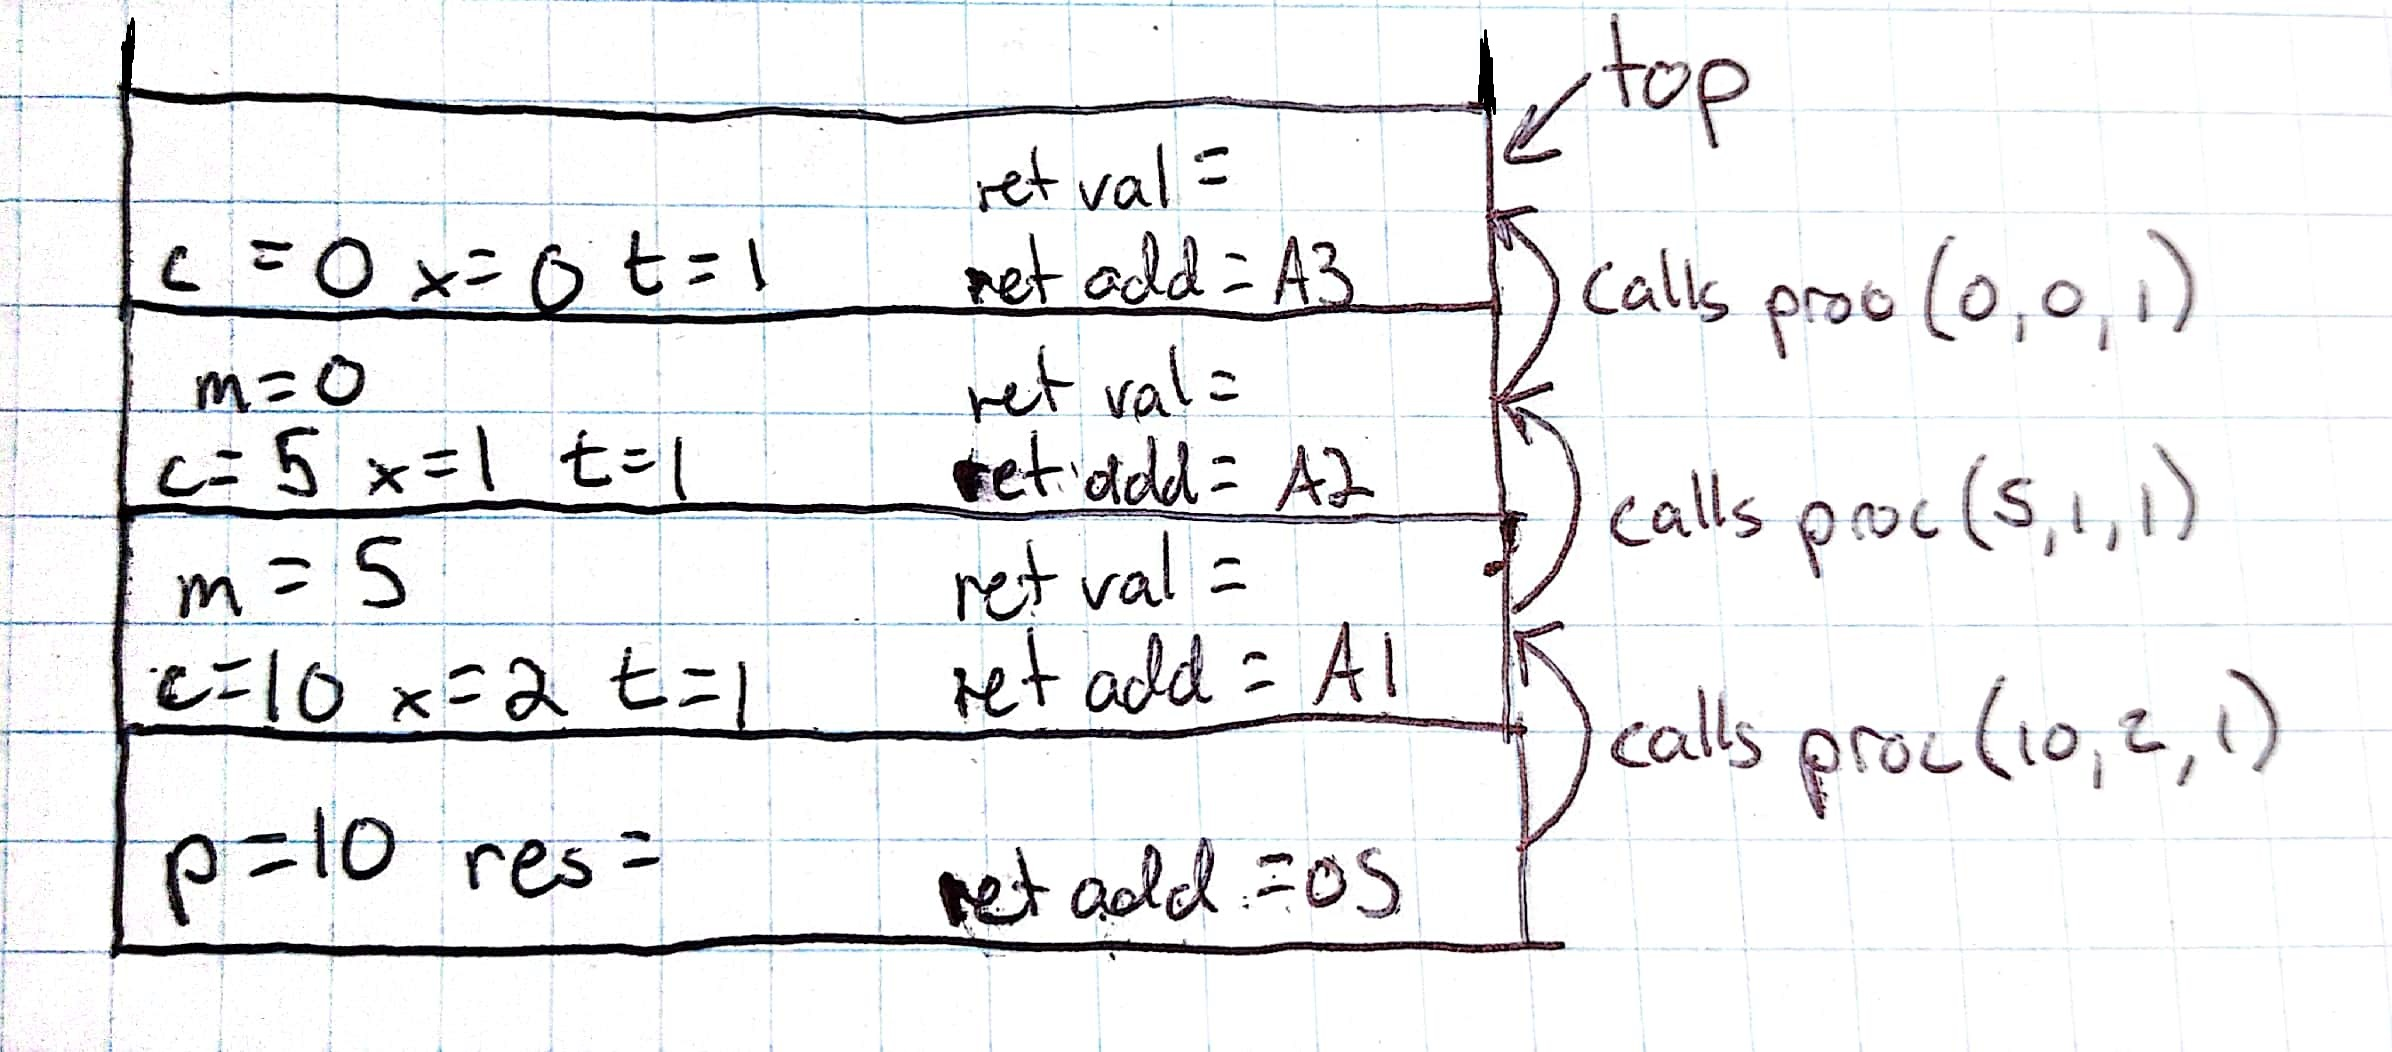
\includegraphics[scale=0.18]{execution stack.jpg}
    \end{center}

\pagebreak
\subsection*{Question 5}
Write in detailed pseudocode, like the one used in class, an algorithm \texttt{find(r,k,v)} that
receives as input the root \texttt{r} of a tree and two integer values \texttt{k} $\geq$ 0, and \texttt{v}, and it returns the number
of nodes at level \texttt{k} storing the value \texttt{v}. For example, for the tree below with root \texttt{r} the invocation
\texttt{find(r,2,4)} must return the value 2 as there are two nodes as level 2 that store the value 4, the
invocation \texttt{find(r,3,9)} must return 0 as no node at level 3 stores the value 9, and \texttt{find(r,5,4)}
must also return 0 as there are no nodes at level 5 in this tree.

\begin{center}
    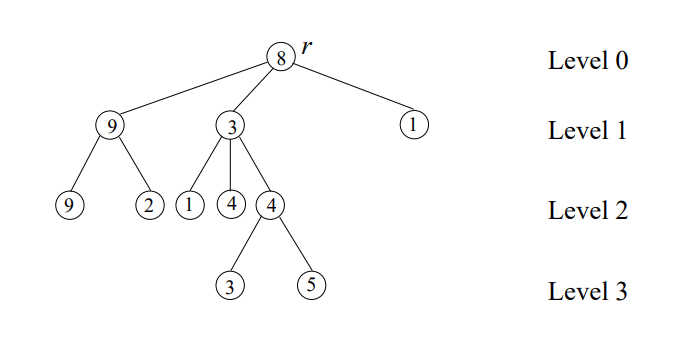
\includegraphics[scale=0.8]{binarytree.PNG}
\end{center}

For a node $r$ let $r$.isLeaf()\footnote[1]{Note: I am assuming that .isLeaf() returns True for the nodes (9, 2, 1, 4, 3, 5, 1) in the above tree - that is, nodes without non-null children} return $true$ if $r$ is a leaf and $false$ otherwise. To get the value stored in a node $r$ use $r$.getValue(). To access the children of a node $r$ use the following pseudocode:\newline
\hspace*{5mm}\textbf{for \textnormal{each child} $c$ \textnormal{of} $r$ do}

Hint. In the initial call to the algorithm the value of the first parameter is the root of the tree and the
value of the second parameter is the target level. Every time that the algorithm is invoked recursively
the value of the second parameter must be updated how?

\pagebreak

\subsubsection*{Pseudocode:}

\textbf{Algorithm:}\texttt{find(r,k,v)}\newline
\textbf{In: }\normalfont{}Root $r$ of a tree, value $k \geq 0$, and value $v$\newline
\textbf{Out: }\normalfont{}Number of nodes at level $k$ storing the value $v$
\begin{align*}    
&\textbf{$count$ $\leftarrow$ 0} &\text{initialize counter}\\
&\textbf{if $r$ \normalfont{is null} \textbf{then return} $0$} &\text{edgecase of root being null}\\
&\textbf{if $k = 0$} &\text{check to see if this is the level we want to check}\\
&\hspace*{5mm}\textbf{if \normalfont{$r$.getValue() = v} \textbf{return} 1} &\text{if this is the right level and data matches, return 1}\\
&\hspace*{5mm}\textbf{return } 0 &\text{if this is the right level and data doesn't match, return 0}\\
&\textbf{else if } r.\textnormal{isLeaf()} = \text{false} &\text{if not the correct level, check if $r$ has children to iterate over}\\
&\hspace*{5mm}\textbf{for \textnormal{each child} $c$ \textnormal{of} $r$ do} &\text{iterate through children nodes}\\
&\hspace*{10mm}\text{count $\leftarrow$ count + find$(c,k-1,v)$}&\text{sums returns from recursive child calls with decremented $k$}\\
&\textbf{return } \textnormal{count}&\text{returns final sum of matching nodes}\\
\end{align*}

\subsection*{Question 6}

Compute the time complexity of the following algorithm. You must explain how many
operations are performed per call, how many calls to the algorithm are made, how many operations
the algorithm performs in total, and what the order of the time complexity is.

Algorithm func($n$) performs $c_1$ log $n$ operations, where $c_1$ is a constant.

\begin{align*}
    &c_2=
    \begin{cases}
    &\textbf{if $r$}\textnormal{ is a leaf }\textbf{then return $n$ + \texttt{func($n$)}}\\
    \end{cases}\\
    &c_3=
    \begin{cases}
    &\textbf{else \textnormal{\{}}\\
    &\textnormal{\hspace*{4mm}$v\leftarrow$\texttt{func($n$)}}\\
    &\textnormal{\hspace*{4mm}$v\leftarrow$$v+$\texttt{algo}\textnormal{($r$.leftChild())$+$}\texttt{algo}\textnormal{($r$.rightChild())}}\\
    &\hspace*{4mm}\textbf{return $v$}\\
    &\text{\}}\\
    \end{cases}
\end{align*}

\pagebreak

Compute the complexity ignoring recursive calls (complexity of one call):\newline
- $c_2+c_1\log n$ if $r$ is a leaf\newline
- $c_3+c_1\log n$ if $r$ is not a leaf

Compute the number of recursive calls:\newline
- Each internal node calls the alogrithm twice\newline
- Leaf nodes do not make recursive calls\newline
- There are $\frac{n-1}{2}$ internal nodes in a proper binary tree, so $n-1$ recursive calls are made\newline
- Including the inital call, $n$ calls are made to the algorithm in total

Combine number of calls with the complexity of each call:\newline
- $n$ calls are made, each with a constant amount of operations and a $c_1\log n$ call to func\newline
- We know this will be consolidated to $n\log n$ after removing constants - let's prove it

\begin{align*}
&f(n)=\sum_{leaves}^{}(c_2+c_1\log n)+\sum_{\textit{internal nodes}}^{}(c_3+c_1\log n)\\ 
&f(n)=\sum_{leaves}^{}(c_2)+\sum_{leaves}^{}(c_1\log n) + \sum_{\textit{internal nodes}}^{} (c_3) + \sum_{\textit{internal nodes}}^{}(c_1\log n)\\
&f(n)=leaves*\stkout{c_2}+leaves*c_1\log n+internal*\stkout{c_3}+internal*c_1\log n\\
&f(n)=leaves+internal+(leaves+internal)c_1\log n\\
&f(n)=n+n*\stkout{c_1}\log n\\
&f(n) \text{ is } O(n\log n)
\end{align*}


\end{document}